\section{Methods}
Here I explain Markov brains, the alternate representation I will use in this work, as well as the changes to the patch harvesting environment required to accommodate the new substrate. 

\subsection{Markov brains}

% What are Markov brains?
At their most abstract level, the substrates we evolve on interactive tasks need three things: a way to receive inputs, a way to process data, and a way to output data. 
Avida organisms handle each of these with instructions, including specialized instructions for each environment to facilitate inputs and outputs. %some of which are specifically designed to pull information from the environment or take an action. 
Here we use Markov brains, which process data via binary logic gates connected to input and output buffers \citep{hintzeMarkovBrainsTechnical2017}. 


\begin{figure}[h!]
    \centering
    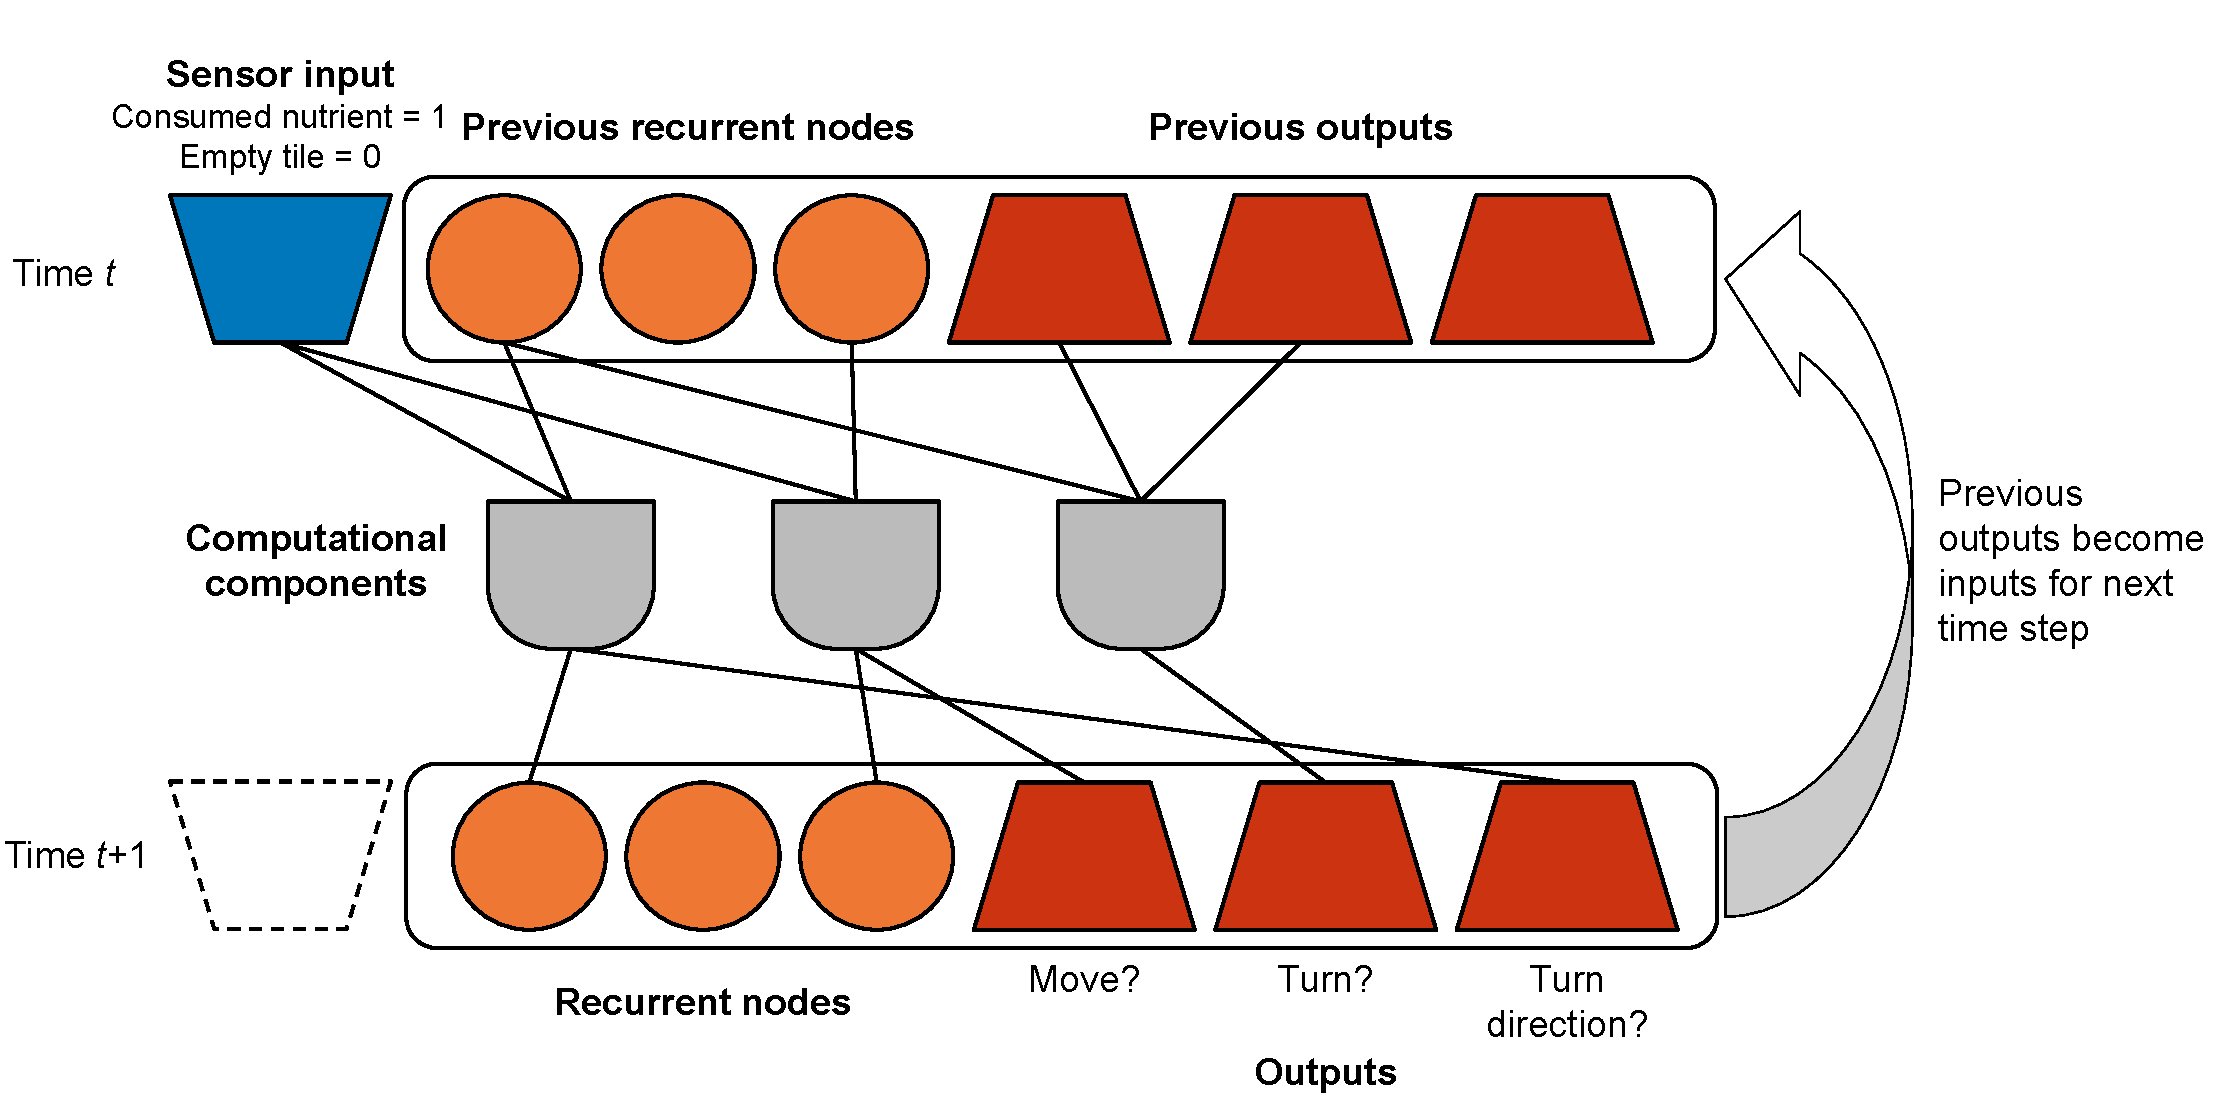
\includegraphics[width=0.95\textwidth]{07_potentiation_across_representations/media/markov_brain_conceptual_figure.pdf}
    \caption{Conceptual diagram of a Markov brain with inputs and outputs for the patch harvesting task, adapted from \citep{hintzeMarkovBrainsTechnical2017}.
    The single input, corresponding to the type of tile the organism is on, is shown as a blue trapezoid. 
    This example has three recurrent nodes (shown as orange circles) and three computational components (shown in gray). 
    The patch harvesting environment has three outputs, shown here as red trapezoids. 
    Note that the recurrent and output nodes (i.e., those in the rounded rectangle) will be passed as input in the next time step.
    The sensor input must come from the environment, as shown by the dashed trapezoid in the \textit{t+1} buffer.}
    \label{fig:varying_representations:markov_brain}
\end{figure}

% Go into more detail on how the brains work? Encoding?
Figure \ref{fig:varying_representations:markov_brain} shows an example Markov brain in the patch harvesting environment. 
At a given timestep \textit{t}, the organism will receive one input, some number of recurrent nodes, and three outputs (inputs and outputs described in the next subsection).
The genome of a particular brain encodes some number of computational components, including which inputs and outputs they are connected to. 
The inputs at timestep \textit{t} are passed into these computational components, and the outputs are written into an output buffer that includes recurrent nodes and output nodes (i.e., actuators). 
The environment will read the outputs and perform the appropriate actions, as described below. 
Finally, the recurrent and output nodes are passed back to the brain as part of the input buffer for time \textit{t+1}. 
This process constitutes one update, and each Markov brain will be executed for a given number of updates in order to perform its actions in the environment. 
A full description of Markov brains is available in \citep{hintzeMarkovBrainsTechnical2017}.

Computational components perform the transformation of inputs to outputs at each timestep. 
Here, I will only use deterministic logic gates for computational components, as they should be sufficient given that memory is already available via recurrent nodes. 
These logic gates take in some number of inputs and produce some number of outputs, with each deterministic logic gate containing its own truth table to map from inputs to outputs. 
For a given Markov brain, its computational components are all encoded in its genome. 
While we will avoid the details of the encoding (see \citep{hintzeMarkovBrainsTechnical2017} for details on computational components, logic gates, and the encoding scheme), it is important to note that Markov brains use a genetic encoding as compared to Avida's direct encoding. 
This allows for more flexibility in what effects mutations can have in a Markov brain. 
In our previous Avida work, a mutation always adds, removes, or swaps a single instruction. 
Mutations in Markov brains can have more minute difference, such as changing the type of computational component, modifying input/output connections, or changing the truth table of a logic gate. 
Combined with the fact that many sites in a Markov brain can be non-coding, these genomes have many possibilities for neutral and nearly-neutral mutations.
Additionally, the different effects that mutations can have create many a different suite of potential epistatic interactions than those found in Avida. 
Since we expect that epistatic interactions play a key role in the potentiation of a genome, these differences will likely influence how potentiation changes in Markov brains. 

\subsection{Changes to the patch harvesting environment and evolution system}

% We can't just throw Markov brains in the environment, we need to make a few changes
In Avida, the patch harvesting environment adds four new instructions: \texttt{Turn Left}, \texttt{Turn Right}, \texttt{Move Forward}, and \texttt{Sense}.
These instructions allow the organisms to pull information from the environment and take actions. 
Since Markov brains do not operate on the basis of instructions, we need to make some modifications to how the environment handles inputs and outputs. 

% How to modify IO
Instead of a \texttt{Sense} instruction that pulls the current tile's information into a register, to support Markov brains we will place the current tile's cue in the input buffer. 
Avida organisms work on 32-bit integers while Markov brains work on binary signals, so we will also need to convert the data itself. 
Because organisms consume food when they move on a tile, they can only encounter two types of tile cues: an empty tile or a tile that previous had food that has since been consumed. 
As such, we will place a one in the organism's input buffer if the tile previously contained food, or a zero if the tile has always been empty. 
Similarly, we need to determine what actions the organism will take based on the output buffer. 
To do this, we will give the organisms three bits of output. 
The first bit corresponds to movement; the organism will move forward if the movement bit is set. 
The last two bits will be used for turning. 
The first turning bit will determine if the organism will turn, while the second turning bit will determine which direction the organism will turn. 
Turning will be overridden by moving. 
Using two different bits to determine if the organism moves and if it turns allows for time steps with no environmental actions taken while still performing computation into the memory bits. 
With these modifications, the Markov brain organisms will have the pieces to sense their environment, do computation using normal Markov brain gates, and perform actions via their outputs. 

% Evolution system now needs to be synchronous 
The scoring of the environment and the classification of behaviors does not need to change from the Avida implementation. 
Organisms will still be rewarded for consuming food and punished for wandering into empty tiles. 
However, the evolution system itself will need to change to accommodate the change in representation. 
Avida operates on the concept of asynchronous generations -- organisms replicate themselves by executing certain instructions. 
This concept does not exist in Markov brains, so they must be externally replicated. 
As such, the Markov brains will evolve in a synchronous generation system. 
All organisms in the population will be evaluated independently to calculate their scores. 
Once the scores have been collected, we will select parents for the next generation by applying roulette (fitness proportional) selection, as it is the most similar to how Avida doles out updates. 
After replicating the parents and applying mutations, we will have our next generation and can restart the process.
We will conduct some preliminary experiments to ensure that Markov brains receive a comparable amount of time in the environment and comparable number of generations to the Avida organisms of Chapter \ref{chap:varying_environments}.

